\documentclass[a4paper]{article}
\usepackage[latin1]{inputenc}
\usepackage[T1]{fontenc}
\usepackage[francais]{babel}
\usepackage{entete}
\usepackage{noitemsep}
\usepackage{euscript} 
\usepackage{amsmath,amssymb,amsfonts,amsthm}
\usepackage{graphicx,graphics,epsfig,subfigure,color}
\usepackage{url}
%\usepackage{algorithm2e}
\usepackage{multicol}
\usepackage{a4wide}
\usepackage{latexsym}
\usepackage{verbatim}
\setlength{\textheight}{23.5cm}
\setlength{\topmargin}{-1cm}
\setlength{\textwidth}{155mm}
\setlength{\oddsidemargin}{2mm}

%\renewcommand{\baselinestretch}{0.85}

%\input{macroAlgo}
%\dontprintsemicolon

\setlength{\parindent}{0pt}  %%suppression indentation


\begin{document}
\selectlanguage{francais}
\author{D. Fourer, L. Lagon}
\newcommand{\universityname}{IUT d'\'Evry Val d'Essonne}
\newcommand{\deptname}{D\'epartement TC (S3)}
\newcommand{\years}{2023-2024}

%------------------- TITRE -----------------------------------------
\date{Septembre 2023} 
\TDHead{\universityname}{\deptname}{R3.12, \years}{\large TD4: Fonctions avanc\'ees d'un tableur}
%\TDHead{DUT TC}{}{\large TIC3: Fonctions avanc\'ees d'un tableur}
%-------------------------------------------------------------------

%% formule avec  SI / ET / OU imbriques
\vspace{-0.2cm}
% EQUIV / INDEX
Fonctions utiles:
\begin{itemize}
% \item Tableau: ensemble de cellules d\'efini par une plage de valeurs (e.g. A1:D5)
 \item \verb? INDEX(tableau; no_ligne ; no_colonne)? \\Retourne la valeur d'une cellule dans un tableau aux coordonn\'ees \verb?(no_ligne,no_colonne)?.
 \item \verb? EQUIV(valeur_recherche; plage_de_recherche; 0) ?\\ Recherche une valeur dans un tableau et retourne sa position.
 (Le 0 peut etre remplac\'e par -1 ou 1 pour rechercher une valeur approch\'ee de \verb?valeur_recherche? plus petite ou plus grande).
 \item \verb? SI(condition;si_vrai;si_faux)?. Teste une condition et retourne le r\'esultat correspondant.
 \item \verb? ET(condition1;condition2)? Retourne VRAI si les 2 conditions sont vraies.
 \item \verb? OU(condition1;condition2)? Retourne VRAI si au moins une des 2 conditions est vraie.
\end{itemize}

%~\par{}
%% source http://www.formulecredit.com/mensualite.php
\exost L'objectif de cet exercice est de cr\'eer un simulateur de pr\^ets immobiliers.\\
En disposant d'une base de donn\'ees de clients et de taux, vous proposerez une interface permettant 
de calculer automatiquement les frais qui s'appliquent \`a une situation ainsi que le montant des
mensualit\'es.
\begin{enumerate}
 \item R\'ecup\'erez le fichier \url{https://fourer.fr/Ens/2324/RCN3/pret_immo.zip} et ouvrez le.
 \item Cr\'eez la feuille ci-dessous qui calcule automatiquement tous les champs attendus:\\ % \`a l'aide des formules ad\'equates: %\centering\includegraphics[width=0.6\textwidth]{calc.jpg}
 \includegraphics[width=0.8\textwidth]{img/calc.jpg}
\end{enumerate}
\underline{Indications:} Vous utiliserez les fonctions INDEX et EQUIV pour rechercher des valeurs dans les autres feuilles de calcul.
On supposera un pr\^et \`a remboursement constant dont les mensualit\'es $m$ (avec int\'er\^ets) se calculent par:
\begin{equation}
 m = \frac{C \times t_m}{1 - (1+t_m)^{-d}}
\end{equation}
avec $C$ le capital emprunt\'e, $t_m=\frac{t}{12}$ le taux mensuel (avec $t$ le taux d'int\'er\^et) et $d$ la dur\'ee en mois du pr\^et.
Le co\^ut de l'assurance se calcule en appliquant le taux sur la somme totale emprunt\'ee divis\'ee par 12 mois.
Le total des frais d'assurance correspond \`a la somme cumul\'ee des mensualit\'es vers\'ees durant toute la dur\'ee du pr\^et.
%N'h\'esitez pas \`a ajouter des cellules n\'ecessaires permettant de faire tous les calculs interm\'ediaires.
%\vspace{-0.5cm}

\begin{flushleft} % https://support.office.com/fr-fr/article/charger-le-compl%C3%A9ment-solveur-dans-excel-612926fc-d53b-46b4-872c-e24772f078ca
\exost En utilisant le solveur (fonction compl\'ementaire \`a ajouter via: options/compl\'ement/atteindre),
trouvez \textbf{le nombre de mensualit\'es optimal} minimisant
tous les frais li\'es au pr\^et (int\'er\^ets et assurance cumul\'es) tel que le montant 
\`a rembourser chaque mois (hors assurance) ne d\'epasse pas 33\% des revenus du client.
\end{flushleft}
\vspace{-0.4cm}
\centering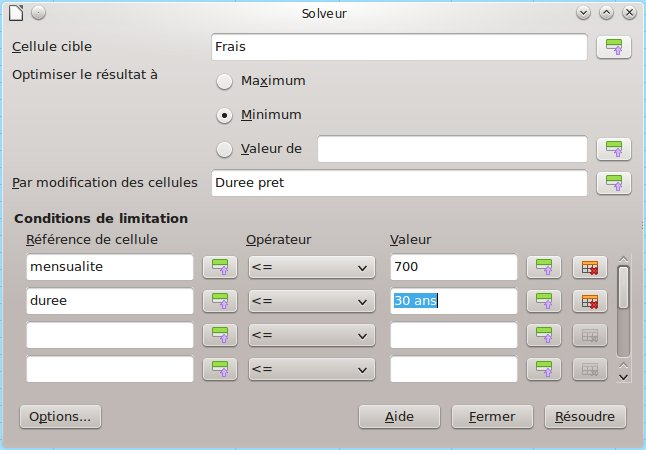
\includegraphics[width=0.45\textwidth]{img/solveur.jpg}\\
\flushleft \textbf{Bonus:} Utilisez le solveur pour calculer les mensualit\'es pour un pr\^et \`a taux annuel (les int\'er\^ets sont calcul\'es sur le capital d\^u en d\'ebut d'ann\'ee).

\end{document}

% End Of File

